\documentclass[12pt,a4paper]{article}

% Paquetes básicos
\usepackage[utf8]{inputenc}
\usepackage[T1]{fontenc}
\usepackage[spanish]{babel}
\usepackage{amsmath, amssymb}
%\usepackage{siunitx} % Ángulos
\usepackage{graphicx}
\usepackage{float}
\usepackage{geometry}
\usepackage{xcolor}
\geometry{margin=2.5cm}
\usepackage{array}
\usepackage{longtable}
\usepackage{hyperref}
\usepackage{caption}
\usepackage{subcaption}
\usepackage{setspace}
\usepackage{multirow}
%\usepackage{minted}  % Códigos
%\usepackage{gensymb} % Grados: "°"
\usepackage[backend=biber, style=ieee]{biblatex}
\usepackage{csquotes}
\usepackage{booktabs}
\addbibresource{Bibliografía.bib}
\graphicspath{{Figuras/}}
\onehalfspacing
\hypersetup{
    colorlinks  = true,
    linkcolor   = blue,    
    citecolor   = blue,
    urlcolor    = blue,
    filecolor   = blue
}


\begin{document}       
\renewcommand{\figureautorefname}{Fig.}
\renewcommand{\tableautorefname}{Tab.}
\renewcommand{\equationautorefname}{Ec.}


% Carátula personalizada
\begin{titlepage}
    \centering
    
\includegraphics[width=0.7\textwidth]{Marvell Logo.png}\\[1.5cm]

    {\Large \textbf{PROGRAMA DE FORMACIÓN MARVELL} \\[0.5cm]}
    {\Large Diseño Digital para Sistemas DSP} \\[0.5cm]

    \rule{\textwidth}{0.5pt} \\[0.5cm]
    {\Large \textbf{Ejercicios Módulo 6: Planificación Temporal} \\[0.3cm]}
    \rule{\textwidth}{0.5pt} \\[1cm]
    
\vfill
\begin{tabular}{l l}
    \textbf{Profesor:} & Del Barco, Martín.\\
    \\[0.5cm]
    \textbf{Alumnos:} & Monja, Ernesto Joaquín\\
                      & Zúñiga, Guillermo Rubén Darío\\
\end{tabular} \\[5cm]
\vfill
{\centering Año 2026 \par}

\end{titlepage}



% Índice
\tableofcontents
\newpage



\section{Introducción}                                              \label{sec_1}
El presente informe tiene como objetivo analizar y aplicar los conceptos de planificación temporal sobre la arquitectura de un filtro FIR directo de 4 coeficientes. Para ello, se empleó la representación formal mediante \emph{Grafos de Flujo de Datos} (DFG), identificando nodos, aristas y elementos de retardo (registros). Sobre este modelo, se aplicaron técnicas de \emph{scheduling} y se exploraron dos estrategias contrapuestas: una implementación iterativa basada en el reuso de recursos y el método de \emph{pipelining} para minimizar el camino crítico. Todo esto para evaluar y comparar el \emph{PPA} entre ambas soluciones. Finalmente, se evalúa el \emph{límite de iteración} (IPB) introducido por la realimentación en una topología IIR, y cómo varía al aplicar la técnica de \emph{C-Slow}.




\section{Desarrollo}                                                \label{sec_2}
\subsection{Data Flow Graph de un \textit{FIR}}                     \label{sec_2.1}
Un filtro \textit{FIR} de 4 coeficientes (taps) en forma directa se describe matemáticamente mediante la ecuación de diferencias presentada en la \autoref{eq_1}.
\begin{equation}
    y[n] = h_{0} x[n] + h_{1} x[n-1] + h_{2} x[n-2] + h_{3} x[n-3]
    \label{eq_1}
\end{equation}

En la \autoref{fig:fig_1} podemos apreciar la estructura en forma de \textit{DFG} (Data Flow Graph).
\begin{figure}[H]
    \centering
    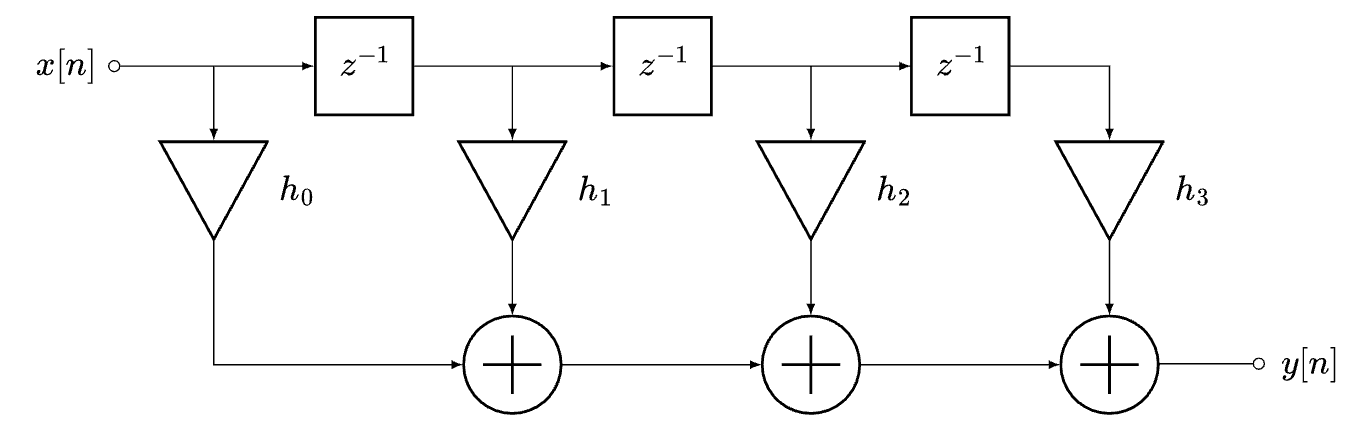
\includegraphics[width=1\linewidth]{Figura 1.PNG}
    \caption{\textit{DFG} de un filtro \textit{FIR}. \cite{b2}}
    \label{fig:fig_1}
\end{figure}

En esta figura podemos apreciar los siguientes elementos del \textit{DFG}:
\begin{itemize}
    \item \underline{Nodos (Operaciones):} El grafo contiene $4$ multiplicadores (correspondientes a la multiplicación por los coeficientes $h_{0}, h_{1}, h_{2}$ y $h_{3}$) y $3$ sumadores encargados de acumular los productos.
    \item \underline{Aristas (Dependencias):} Son las conexiones que dirigen los datos desde la señal de entrada $x[n]$ hacia los multiplicadores, y las salidas de estos hacia la cadena de sumadores.
    \item \underline{Registros ($z^{-1}$):} Se necesitan $3$ registros de retardo ubicados secuencialmente en la línea de entrada para almacenar los valores históricos $x[n-1], x[n-2]$ y $x[n-3]$.
\end{itemize}





\subsection{\emph{Scheduling ASAP} y \emph{ALAP}}                   \label{sec_2.2}
El método de \emph{scheduling} consiste en definir los instantes en los que cada operación de un grafo se debería ejecutar, respetando dos tipos de restricciones: de dependencia, donde una operación solo puede ejecutarse cuando sus operandos estén disponibles; y de recursos, donde el número de sumadores, multiplicadores, etc. es finito. Dentro de este método existen dos estrategias:
\begin{itemize}
    \item \underline{ASAP} (As Soon As Possible): Cada operación se ejecuta lo antes posible. De aquí se obtiene la latencia total del circuito.
    \item \underline{ALAP} (As Late As Possible): Cada operación se ejecuta lo más tarde posible, pero sin afectar la latencia total. En este caso se descubre la flexibilidad temporal de cada operación
\end{itemize}

Con estos dos enfoques, se realizó el \textit{scheduling} del filtro \textit{FIR} de la \autoref{sec_2.1}. Este caso se muestra en la \autoref{fig:fir_scheduling}, donde se propone que un sumador tiene una latencia de $1 \, ut$ (1 unidad de tiempo), mientras que un multiplicador tiene una de $2 \, ut$. El \textit{scheduling ASAP} se encuentra en la \autoref{fig:fir_asap}, y se observa que el camino crítico (1 multiplicador y 3 sumadores) tiene una latencia de $4 \, ut$, por lo que esta es la latencia total. Luego, el \textit{scheduling ALAP} de la \autoref{fig:fir_alap} muestra que los únicos operadores flexibles son $M_{2}$ y $M_{3}$.
\begin{figure}[H]
    \centering
    \begin{minipage}{0.48\linewidth}
        \centering
        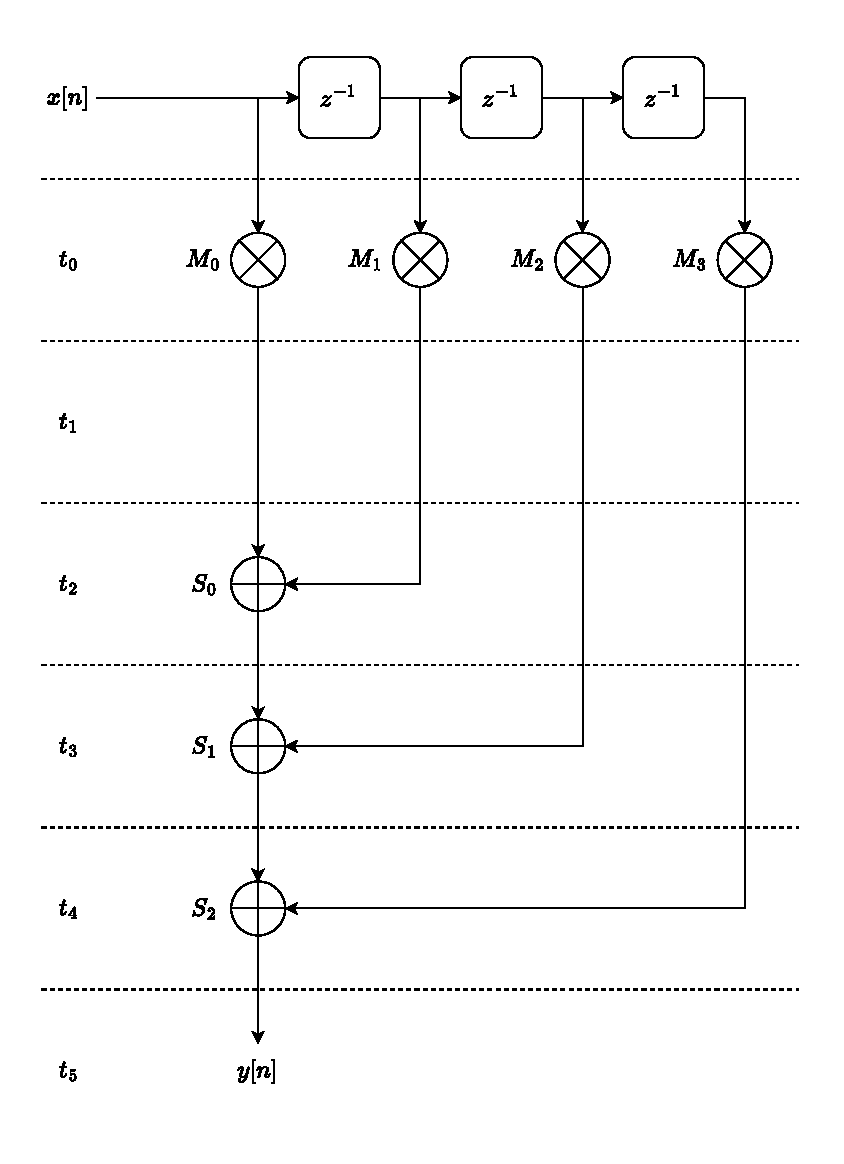
\includegraphics[width=\linewidth]{Figuras/fir_asap.pdf}
        \subcaption{Método \textit{ASAP}.}
        \label{fig:fir_asap}
    \end{minipage}
    \hfill
    \begin{minipage}{0.48\linewidth}
        \centering
        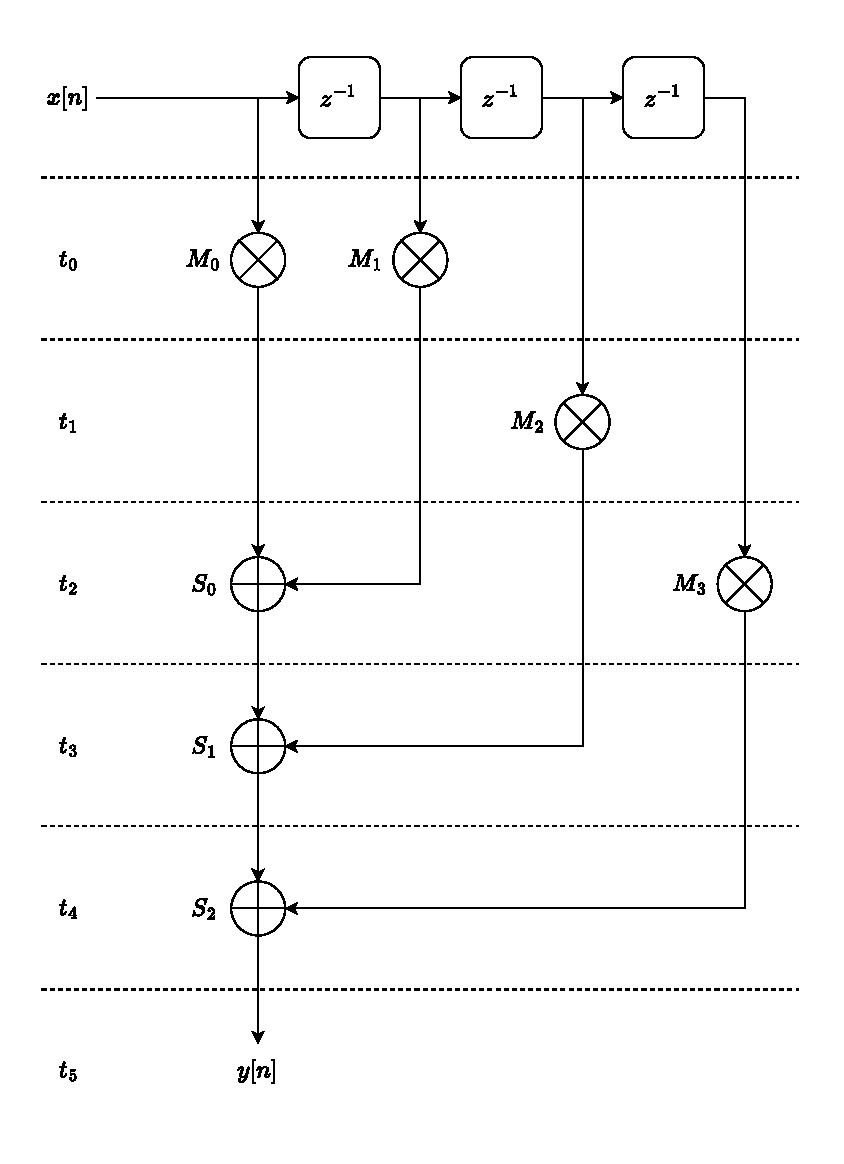
\includegraphics[width=\linewidth]{Figuras/fir_alap.pdf}
        \subcaption{Método \textit{ALAP}.}
        \label{fig:fir_alap}
    \end{minipage}
    \caption{\textit{Scheduling} del filtro \textit{FIR} de $4$ coeficientes.}
    \label{fig:fir_scheduling}
\end{figure}

Se calculó la movilidad de $M_{2}$ y $M_{3}$, resultando
\begin{equation}
    \begin{cases}
        m_{M2} = 1 - 0 = 1 \\
        m_{M3} = 2 - 0 = 2
    \end{cases}
    \label{eq_2}
\end{equation}

Nótese que la movilidad de ambos multiplicadores no cambiaría si se modifica su latencia con respecto a los sumadores.



\subsection{Versión Iterativa con \textit{MAC}}                     \label{sec_2.3}
Al restringir los recursos a \textbf{1 sumador y 1 multiplicador}, estamos aplicando la técnica arquitectónica de \textit{Folding}, reutilizando el \textit{HW} en distintos ciclos temporales.

Veamos primero como es el proceso de diseño de la máquina de estados (\textit{FSM}): Dado que procesar una muestra requiere $4$ multiplicaciones y $3$ sumas, al contar con un único bloque \textit{MAC} (Multiplicador-Acumulador), necesitamos obligatoriamente un mínimo de $4$ ciclos de clock. La \textit{FSM} contará entonces con $4$ estados iterativos para computar cada salida $y[n]$:
\begin{enumerate}
    \item \underline{Ciclo 1 ($S_{0}$):} Se enruta $x[n]$ con $h_{0}$ a través de MUXes (Operación: $A_{cc} = h_{0} \cdot x[n]$).
    \item \underline{Ciclo 2 ($S_{1}$):} Se enruta $x[n-1]$ con $h_{1}$ (Operación: $A_{cc} = A_{cc} + (h_{1} \cdot x[n-1])$).
    \item \underline{Ciclo 3 ($S_{2}$):} Se enruta $x[n-2]$ con $h_{2}$ (Operación: $A_{cc} = A_{cc} + (h_{2} \cdot x[n-2])$).
    \item \underline{Ciclo 4 ($S_{3}$):} Se enruta $x[n-3]$ con $h_{3}$ donde se entrega el resultado a la salida y se resetea el acumulador para la próxima muestra (Operación: $y[n] = A_{cc} + (h_{3} \cdot x[n-3])$).
\end{enumerate}

Este proceso se muestra gráficamente en la \autoref{fig:fig_2}.
\begin{figure}[H]
    \centering
    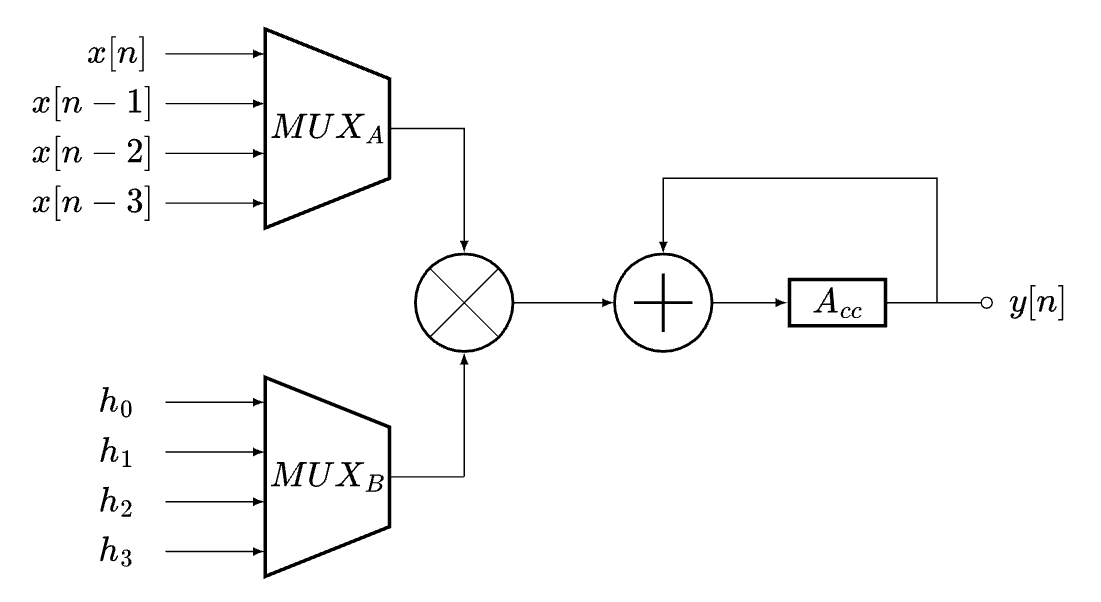
\includegraphics[width=0.7\linewidth]{Figura 2.PNG}
    \caption{\textit{FSM} de la versión iterativa del \textit{FIR}.}
    \label{fig:fig_2}
\end{figure}

Se tienen entonces que las \textbf{Estimaciones Temporales} son:
\begin{itemize}
    \item La \textit{Latencia} es de: $4 \, [\text{ciclos}]$ (Es el tiempo total desde que ingresa la muestra $x[n]$ hasta que se produce la salida $y[n]$).
    \item El \textit{Throughput} es de $0.25 \, [\frac{\text{muestras}}{\text{ciclo}}]$ (se genera 1 resultado válido cada 4 ciclos de clock).
\end{itemize}



\subsection{\emph{Feed-Forward Cut-Set}}                       \label{sec_2.4}
El método \emph{Feed-Forward Cut-Set} consiste en dividir un grafo en $2$ partes, trazando una linea que corta un conjunto de aristas que van a la misma dirección (no hay bucles), y luego agregando una cierta cantidad de registros en medio, con el objetivo de reducir el camino crítico.

Esta técnica se realizó sobre el filtro \textit{FIR}, resultando en $2$ etapas de \textit{pipeline} como se muestra en la \autoref{fig:fir_cutset}. Con esto, se logró un camino crítico de $2 \, ut$ ($3 \, ut$ menos que sin \textit{pipeline}) correspondiente a los multiplicadores $M_{0}, ..., M_{3}$ y los dos sumadores $S_{1}$ y $S_{2}$.
\begin{figure}[H]
    \centering
    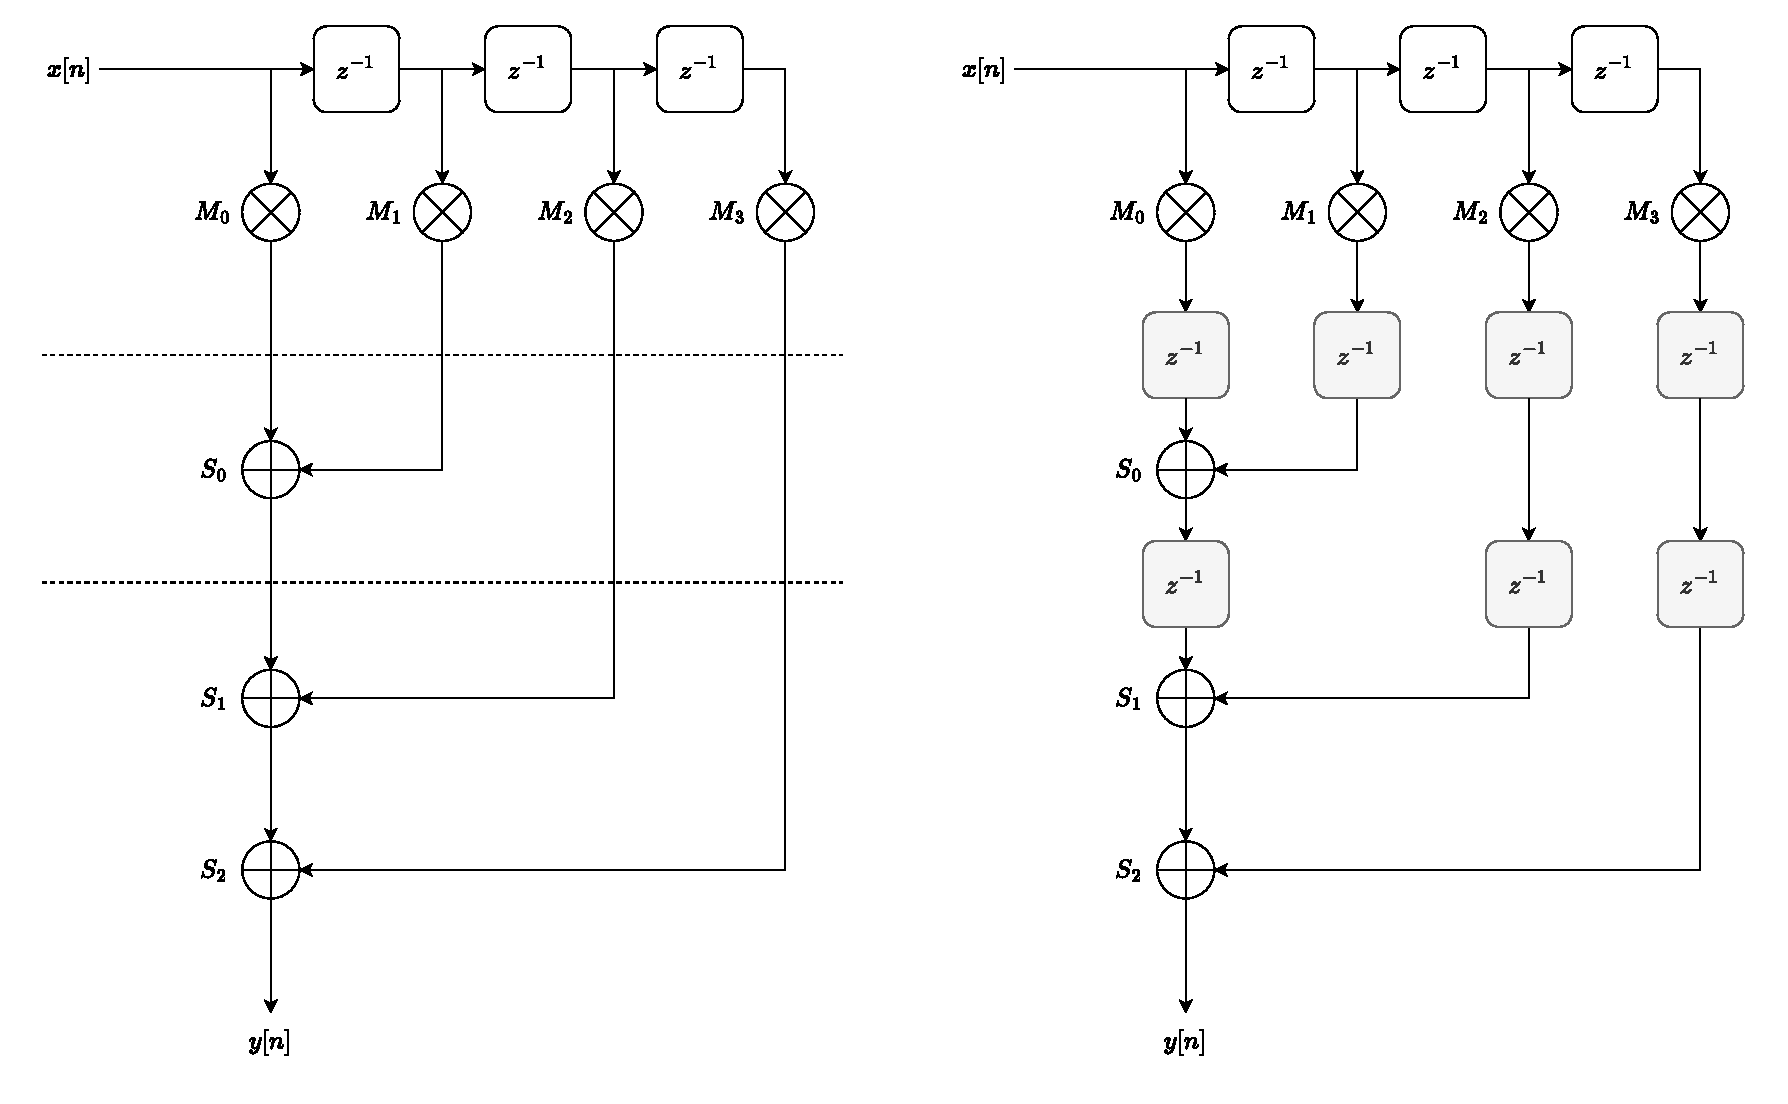
\includegraphics[width=0.85\linewidth]{Figuras/fir_cutset.pdf}
    \caption{Filtro \textit{FIR} con $2$ etapas de \textit{pipeline} mediante el método \textit{Cut-Set}.}
    \label{fig:fir_cutset}
\end{figure}

En la \autoref{tab:cutset} se compara entonces la arquitectura con y sin \textit{pipeline}, asumiendo $1 \, [ut] = 1 \, [ns]$, y se concluye que este método de \textit{retiming} permite utilizar una frecuencia de reloj más alta para el diseño, pero a coste de aumentar la latencia, consumo y área debido al agregado de registros.
\begin{table}[H]
    \centering
    \begin{tabular}{|l|c|c|} \hline
        \textbf{} & \textbf{Sin pipeline} & \textbf{Con pipeline} \\ \hline
        Camino crítico $[ns]$ & 5 & 2 \\
        Frecuencia máxima $[MHz]$ & $\sim 200$ & $\sim 500$ \\
        Latencia [ciclos de reloj] & 0 & 2 \\
        \hline
    \end{tabular}
    \caption{Comparación entre filtro FIR sin pipeline y con pipeline.}
    \label{tab:cutset}
\end{table}


\subsection{Comparación del \textit{PPA}}                           \label{sec_2.5}
Para este análisis \textit{PPA} (Power, Performance, Area) contrastamos la \textbf{Versión Iterativa} (véase la \autoref{sec_2.3}) contra la \textbf{Versión Pipeline} (véase la \autoref{sec_2.4}) insertando etapas de registros para obtener la \autoref{tab:tab_2}.
\begingroup
    \footnotesize
     \begin{longtable}
        {|>{\centering\arraybackslash}m{2.5cm}
         |>{\centering\arraybackslash}m{6cm}
         |>{\centering\arraybackslash}m{6cm}|} \hline
        \textbf{Métrica PPA} & \textbf{Versión Iterativa (Folding)} & \textbf{Versión Pipeline (Unfolded)} \\ \hline
        \endfirsthead
                
        \multicolumn{3}{c}{\textit{Continuación de la página anterior}} \\ \hline
        \textbf{Métrica PPA} & \textbf{Versión Iterativa (Folding)} & \textbf{Versión Pipeline (Unfolded)} \\ \hline
        \endhead
                
        \hline 
        \multicolumn{3}{c}{\textit{Continúa en la página siguiente...}} \\
        \endfoot
                
        \hline
        \caption{Comparativa de recursos y métricas de tiempo (PPA) entre arquitecturas FIR.}
        \label{tab:tab_2}
        \endlastfoot

        \textbf{Latencia} & 4 ciclos & 2 ciclos (según \autoref{tab:cutset}) \\ \hline
        
        \textbf{Throughput} & 0.25 muestras/ciclo (Bajo) & 1 muestra/ciclo (Alto a $\sim 500$ MHz) \\ \hline
        
        \textbf{Área Estimada} & \textbf{Baja:} 1 Mul, 1 Add, MUXes y lógica FSM. & \textbf{Alta:} 4 Mul, 3 Add, y abundantes registros ($z^{-1}$) por el \textit{cut-set}. \\ \hline
        
        \textbf{Consumo} & \textbf{Bajo:} Ideal para bajo consumo; menor conmutación. & \textbf{Alto:} Gran cantidad de hardware combinacional y registros activos. \\ \hline
    \end{longtable}
\endgroup

Se tiene que la planificación define el consumo y área sin tocar la matemática subyacente del algoritmo. La arquitectura iterativa aplica multiplexación en el tiempo, ahorrando área de silicio y reduciendo la potencia dinámica, lo que la hace idónea para sistemas embebidos de bajo consumo y baja velocidad. Por el contrario, la versión con \textit{pipeline} disminuye el camino crítico de $5 \, [ns]$ a $2 \, [ns]$, mejorando sustancialmente el paralelismo y garantizando $1$ resultado por ciclo a una frecuencia máxima mucho mayor, a expensas de un incremento en la latencia inicial, área y consumo.




\subsection{Límite de Iteración (\emph{IPB})}                       \label{sec_2.6}
El \emph{límite de iteración} (\emph{IPB}) es una métrica utilizada para obtener el mínimo período alcanzable en un diseño, y para obtenerlo se debe realizar lo siguiente:
\begin{enumerate}
    \item Identificar los lazos, es decir, los caminos del \textit{DFG} que salen de un nodo y vuelven al mismo nodo, recorriéndolo en sentido dirigido.
    \item Sumar las latencias de todos los nodos del lazo ($T$).
    \item Contar la cantidad de registros sobre ese lazo ($D$).
    \item Calcular el \emph{límite de lazo} para cada lazo $i$ como $LB_{i} = T_{i} / D_{i}$.
    \item El $LB_{i}$ más alto es el $IPB$.
\end{enumerate}

Se puso en práctica este método convirtiendo el filtro \textit{FIR} en un filtro \textit{IIR} de $1^{er}$ orden, utilizando la aproximación de Padé. Mientras que el \textit{FIR} tiene la forma que se muestra en la \autoref{eq_1}, se tiene que el filtro \textit{IIR} termina siendo:
\begin{equation}
    y[n] = \frac{h_{2}}{h_{1}} y[n-1] + h_{0} x[n] + \left(h_{1} - \frac{h_{0} h_{2}}{h_{1}}\right) x[n-1]
    \label{eq_3}
\end{equation}

Lo que se puede reescribir simplemente como muestra la \autoref{eq_4}.
\begin{equation}
    y[n] = a_{1} y[n-1] + b_{0} x[n] + b_{1} x[n-1]
    \label{eq_4}
\end{equation}

La arquitectura de este \textit{IIR} se muestra en la \autoref{fig:iir}. Teniendo en cuenta que solo existe un nodo en este caso, se obtiene que:
\begin{equation}
    IPB = \frac{T_{0}}{D_{0}} = \frac{3}{1} = 3 \, [ut]
    \label{eq_5}
\end{equation}

\begin{figure}[H]
    \centering
    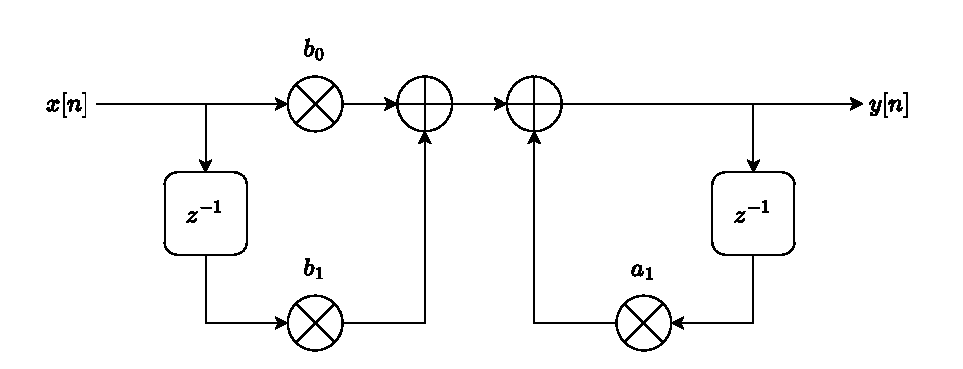
\includegraphics[width=0.8\linewidth]{Figuras/iir.pdf}
    \caption{Esquema del filtro \textit{IIR}.}
    \label{fig:iir}
\end{figure}

Se puede observar que, de todas formas, el camino crítico viene dado por el multiplicador $b_{1}$ y los dos sumadores, pero sobre él se pueden aplicar las técnicas de \textit{pipeline} vistas anteriormente. Luego, suponiendo que el camino crítico está en el lazo, se puede aplicar el método \textit{C-Slow}, que consiste en reemplazar todos los registros del \textit{DFG} por $C$ registros. En la \autoref{fig:iir_cslow} se puede ver este método aplicado al \textit{IIR} con $C = 2$, donde se agregó un registro más al lazo de realimentación y uno al lazo \textit{feed-forward}; a este último se le tuvo que agregar otro registro más para mantener la función de transferencia.
\begin{figure}[H]
    \centering
    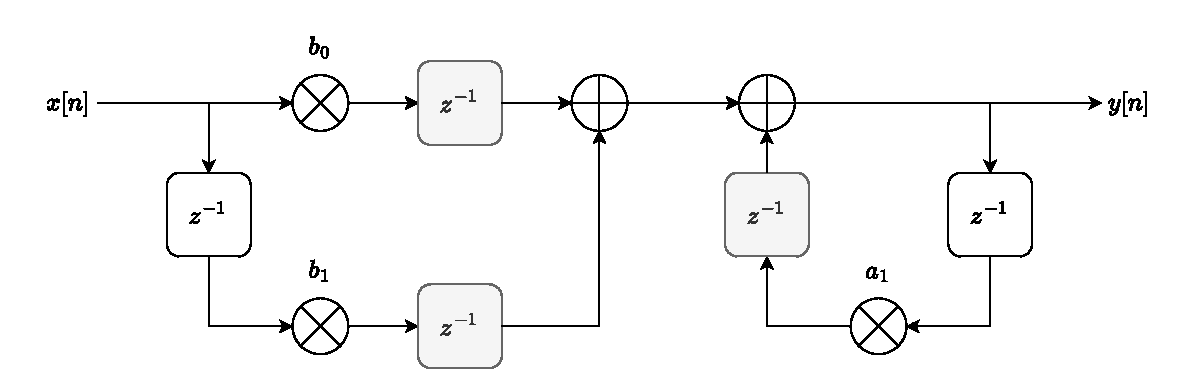
\includegraphics[width=0.8\linewidth]{Figuras/iir_cslow.pdf}
    \caption{\textit{C-Slow} aplicado al filtro \textit{IIR}.}
    \label{fig:iir_cslow}
\end{figure}

Con esto, se obtiene un \textit{IPB} $2$ veces menor:
\begin{equation}
    IPB = \frac{3}{2} = 1.5 \, [ut]
    \label{eq_6}
\end{equation}



\section{Conclusiones}                                              \label{sec_3}
El presente informe demostró cómo la planificación temporal y las transformaciones arquitectónicas impactan directamente en las métricas \textit{PPA} de un sistema \textit{DSP}, sin alterar su matemática subyacente. 

Por un lado, se comprobó que la técnica de \textit{Folding} (arquitectura iterativa) minimiza drásticamente el área (empleando un solo bloque \textit{MAC}) y el consumo a costa de reducir el \textit{throughput}, resultando idónea para sistemas embebidos estrictos. En contraste, el \textit{Pipelining} (mediante \textit{Cut-Set}) permitió elevar la frecuencia máxima a $500 \, [MHz]$ y garantizar $1$ resultado por ciclo, a expensas de un incremento en área y latencia inicial. 

Finalmente, el análisis de sistemas \textit{IIR} evidenció la restricción impuesta por el límite de iteración (\textit{IPB}) en lazos realimentados, el cual logró reducirse a la mitad mediante la técnica \textit{C-Slow}. En definitiva, el diseño de arquitecturas \textit{DSP} no admite una única solución, sino que exige un compromiso de diseño: ya sea priorizar rendimiento (\textit{Pipeline}/\textit{C-Slow}) o priorizar recursos (\textit{Folding}) según los requisitos de cada aplicación.


\newpage
\nocite{*}
\printbibliography[heading=bibintoc, title={4. \ Referencias}]

\end{document}